\documentclass[]{exam}
\usepackage{amssymb}
\usepackage[top=1in, bottom=1.5in, left=1in, right=1in]{geometry}
\usepackage{tikz}
\usepackage{pgfplots}
\checkboxchar{$\Box$}
\usepackage{graphicx}
\usepackage{caption}
\usepackage{float}
\usepackage{enumerate}
\usepackage{comment}
\usepackage{multicol}
\usepackage{color}
\CorrectChoiceEmphasis{\color{red}}
\SolutionEmphasis{\color{red}}
\usepackage{advdate}
\usepackage{gensymb}
\usepackage{mathrsfs}
\usetikzlibrary{arrows}


\usepackage{pgfkeys,pgfcalendar}

\newcount\pgfdatecount
\newcommand{\tomorrow}{%
\pgfcalendardatetojulian{\year-\month-\day+1}{\pgfdatecount}
\pgfcalendarjuliantodate{\the\pgfdatecount}{\myyear}{\mymonth}{\myday}
\pgfcalendarmonthname{\mymonth}\space\myday,\space\myyear%
}


\newcommand{\advanceday}[1][1]{
\begingroup
\AdvanceDate[#1]
\today
\endgroup}

\newcommand{\vertex}{\node[vertex]}
\tikzstyle{vertex}=[circle, draw, inner sep=0pt, minimum size=6pt]

\usepackage{lastpage} 
\usepackage{extramarks}
\usepackage{graphicx} 
\usepackage{tikz}
\usepackage{sectsty} 
\usepackage{amsmath,amsfonts,amsthm} 
\usepackage{wrapfig, blindtext}

% Margins
\topmargin=-0.45in
\evensidemargin=0in
\oddsidemargin=0in
\textwidth=6.5in
\textheight=9.0in
\headsep=0.25in 
\numberwithin{equation}{section}
\linespread{1.1} 
\setlength\parindent{0pt} % Removes all indentation from paragraphs
\setlength\answerskip{-.075in}
\setlength\answerlinelength{.5in}
\newcommand{\myitem}{\part[-]}




% HEADER AND FOOTER
\pagestyle{headandfoot}
\runningheadrule
\runningfootrule
\firstpageheader{Kutztown University}{  }{MATH 181 -- Calculus I}
\firstpageheadrule
\runningheader{Desmos Lab 3}{ }{MATH 181}
\firstpagefooter{}{}{} 
\runningfooter{}{}{Page \thepage\ of \numpages}


\newcommand{\assignmentname}{Desmos Lab III} % Assignment title
\newcommand{\coursetitle}{MATH 181 -- Calculus I}
\newcommand{\duedate}{Due: Tuesday, November 25} % Class/lecture time
\newcommand{\readsections}{Read: Section 4.2 and 4.6} % Teacher/lecturer
\newcommand{\semester}{Fall 2025}
\title{
\vspace{2in}
\textmd{\textbf{\course:\ \assignmentname}}\\
\normalsize\vspace{0.1in}{\duedate}\\
\vspace{0.1in}\large{\textit{\instructor}}
\vspace{3in}
}
\author{\textbf{Author: \authorname}}
\date{Last Updated: \today}

\pointsinrightmargin
\bracketedpoints


%\printanswers % Unomment this line to Print Solutions 

\begin{document}


%%%%%%%%%%%%%%%%%%%%%%%%%%%%%%%%%%%%%%%%%%%%%%%%%%%%%
% TITLES AND SUCH
%%%%%%%%%%%%%%%%%%%%%%%%%%%%%%%%%%%%%%%%%%%%%%%%%%%%%
\hspace{1in}\\ \vspace{.15in}


\hbox to \textwidth{Name: \hrulefill\hrulefill }

\begin{center}
\normalsize
 \fbox{\fbox{\parbox{5.5in}{

        {\bf Instructions:}  All solutions should be prepared carefully and neatly.  Any questions that ask you to explain or justify should have answers written in complete sentences.  All solution sets shall be completed on this packet and handed in at the beginning of class on the due date below.  Careless presentation (e.g.~bad handwriting, pen scribbles, doodles, wasted space, etc) will result in a deduction of points at my discretion.  If the question asks to submit a graph or plot, be sure to print the plot and include it in your final lab report.  Use a PENCIL and if you make a mistake, use an eraser.  Each student should prepare their own solutions that demonstrate their own comprehension of the material.  Submitted work that does not demonstrate clearly the process by which one arrived at the answer will not receive credit of any kind.  Academic dishonesty will not be tolerated. }}}
\end{center}

\vspace{.5cm}

\ifprintanswers
	\begin{center}
		\Huge\textsc{\assignmentname}\\
		\Large{\textsc{\coursetitle}}\\[4pt]
		\Large\textsc{\color{red}Solution Key
		}
	\end{center}
\else
	\begin{center}
		\Huge\textsc{
		\assignmentname}\\[4pt]
                 \Large{\textsc{\coursetitle}\\[10pt]}
                 \Large{\textsc{\duedate}\\[8pt]}
                 \Large{\textsc{\readsections}\\[8pt]
                 }
	\end{center}
\fi


\Large
\begin{center}
\textsc{\textcolor{red}{Solutions}}
\end{center}


%%%%%%%%%%%%%%%%%%%%%%%%%%%%%%%%%%%%%%%%%%%%%%%%%%%%%
%%%%%%%%%%%%%%%%%%%%%%%%%%%%%%%%%%%%%%%%%%%%%%%%%%%%%


\clearpage
%%%%%%%%%%%%%%%%%%%%%%%%%%%%%%%%%%%%%%%%%%%%%%%%%%%%%
% Blank Page
%%%%%%%%%%%%%%%%%%%%%%%%%%%%%%%%%%%%%%%%%%%%%%%%%%%%%
\normalsize
\
\vspace{.5cm}

\huge
\begin{center}
\begin{tabular}{|c|c|c|}
\hline
Problem  & Available  &   Your  \\
Number & Points &    Points  \\	\hline\hline

 $1$  & 10  & \textcolor{red}{10}  \\	\hline
 $2$  & 10  & \textcolor{red}{10} \\	\hline

Total & 20  &\textcolor{red}{20} \\ \hline
\end{tabular}
\end{center}

\pagebreak

\normalsize
\begin{questions}


%%%%%%%%%%%%%%%%%%%%%%%%%%%%%%%%%%%%%%%%%%%%%%%%%%%%
%Part 1
%%%%%%%%%%%%%%%%%%%%%%%%%%%%%%%%%%%%%%%%%%%%%%%%%%%%
\question \underline{The Mean Value Theorem:} In this part, we'll consider a simple function that satisfies the Mean Value Theorem on a general integral.  

\begin{parts}
	\part Open a new graph in Desmos and save it as ``The Mean Value Theorem."
	\part Define the following function on the first line in Desmos: $\displaystyle f(x) = x^3-x$.  On the next two lines, define $a = -2$ and $b = 3$, but allow it to have the slider option.  Graph this function only on the set $[a,b]$ by typing $\{a\leq x \leq b\}$ right next to the function on the first line.  Change the window to $x\in [-3, 4]$ and $y\in [-10, 25]$.  Plot the curve in black with width size 4. 
	\part In the space below, find the secant line slope that connects the points $(-2, f(-2))$ and $(3,f(3))$.  In Desmos, on a new line, define the value $m_{sec}$ to be this slope, but instead of using $-2$ and $3$, define it in terms of $a$ and $b$.  Does Desmos output the same answer that you got?   
	
	\textcolor{red}{The slope of the secant line, $m_{sec}$, over the interval $[-2, 3]$ is given by 
		\begin{align*}
			m_{sec} & = \frac{f(b) - f(a) }{b - a} \\ 
				& = \frac{f(3) - f(-2)}{3 - (-2)} \\ 
				& = \frac{\left[ 3^3 - 3\right] - \left[ (-2)^3 - (-2)\right] }{5} \\ 
				& = \frac{24 + 6}{5} \\ 
				& = \frac{30}{5} \\ 
				& = 6. \end{align*}}
		
	
	\part Create a new folder in Desmos, call it ``Secant Line''.  In this folder, plot the two points $(a,f(a))$ and $(b,f(b)$.  Plot them in orange, size 15, and plot a label with them.  In the space below, derive the equation for the line that connects the two points.  Your answer should only involve $m_{sec}$, $a$, and $f(a)$.  In the folder, define this line and plot it as a dashed green line.  If you change the values of $a$ and $b$, the graph should maintain this line connecting the two points. 
	
	\textcolor{red}{The equation for the secant line in terms of $m_{sec}$, $a$, and $f(a)$ can be found by starting with the point-slope form of a line.  We have
		\begin{align*} 
			y - y_1 = m(x - x_1) \quad & \Rightarrow \quad y - f(a) = m_{sec} (x-a) \\ 
									 & \Rightarrow \quad y = m_{sec}(x-a) + f(a) \end{align*}}
	
	\part Outside the folder, on a new line, define a new slider value $c$ that ranges from $a$ to $b$.  On the line below, define $m_{tan}$ as the slope of the tangent line at $c$ as $m_{tan} = f'(c)$.  
	\part In a new folder called ``Tangent Line,'' plot the point $(c,f(c))$ in red with size 20.  In the space below, write down the equation for the tangent line at $x = c$.  Your answer should only involve $m_{tan}$, $c$, and $f(c)$.  Define this line in the folder and plot it only on the range $[a,b]$. 
	
		\textcolor{red}{Using the same idea as with the secant line, we can find the equation for the tangent line in terms of $m_{tan}$, $c$, and $f(c)$ can be found by starting with the point-slope form of a line.  Letting $m_{tan} = f'(c)$, we have
		\begin{align*} 
			y - y_1 = m(x - x_1) \quad & \Rightarrow \quad y - f(c) = m_{tan} (x-c) \\ 
									 & \Rightarrow \quad y = f'(c)(x-c) + f(c) \end{align*}}
	
	\part Slide the value of $c$ until $m_{tan}$ is the same (or very close) to $m_{sec}$.  What is this value?  In the space below, find the exact value of this number using algebra and calculus.  Show all work.  Once you have the answer, change $c$ to be that value in Desmos to check your answer. 
		
		\textcolor{red}{By sliding the value of $c$, we can see that the desired value is close to 1.5.  To actually solve for this value, we'll set $f'(x) = 3x^2 - 1$ equal to $m_{sec}$ and solve.  We have 
		\begin{align*} 
			3x^2 - 1 = 6 \quad & \Rightarrow \quad x^2 = \frac{7}{3} \\ 
			& \Rightarrow \quad x = \pm \sqrt{\frac{7}{3}}\end{align*}}
		\textcolor{red}{The possible values for $c$ are either $\sqrt{7/3}$ or $-\sqrt{7/3}$.  Since both values are in the interval, we see that both of them have the same slope as the secant line!}
	
		\part When you submit this assignment on D2L, share the url to this graph. 
		
			\textcolor{red}{\texttt{https://www.desmos.com/calculator/9qvyk3h8uf}}

	\vspace{2cm}
	

\end{parts}

\pagebreak






\question \underline{Optimization:} In this part, we'll maximize the area of a fenced in rectangular region given that we only have so much fencing. This will build a code to essentially solve any optimization problem of this form. 

	
\begin{parts}
	\part Open a new graph in Desmos and save it as ``Optimization."
	\part Suppose we have 40 ft of fencing and we wish to enclose a rectangular area $A$.  We want to maximize the area.  Draw a picture below, write down the objective function, and the constraint.  
	
	\textcolor{red}{Let the length and width of the rectangle be $x$ and $y$, respectively as in the figure below.  Then we wish to maximize the area of the function.  Therefore, our objective is function is $A = xy$.  The perimeter, $2x + 2y$, is the amount of fencing, which is constrained to $40$ ft.  Therefore, the constraint equation is $2x + 2y = 40$.  }
	
	\begin{center}
		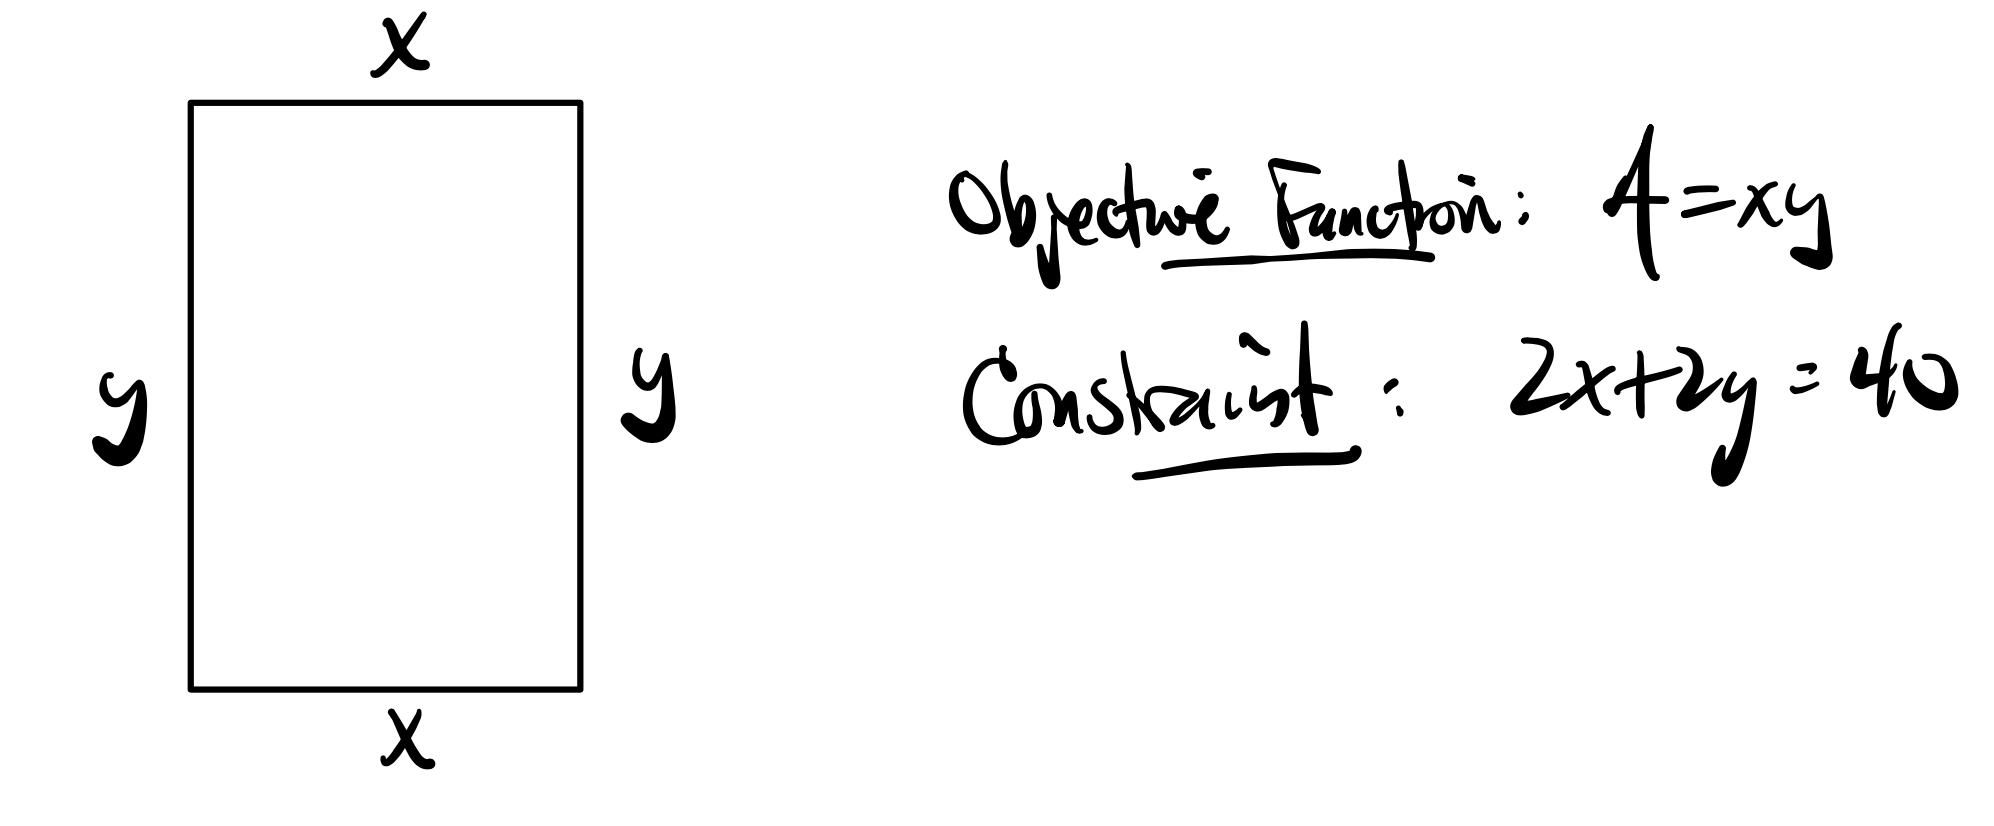
\includegraphics[width = .5\textwidth]{Desmos_Lab_3_Figure.png}
	\end{center}
%	
	\part Use the constraint to eliminate one of your variables and write down the area function as a function of $x$ only below.  Define this function on the first line of Desmos as $A(x)$. Plot it in black and adjust the window so you can see it appropriately.  Does this function have a maximum for positive values of $x$?  Where does it seem to occur? 
	
	\textcolor{red}{We can solve for $y$ in the equation for the constraint: 
		\[ 2x + 2y = 40 \quad \Rightarrow \quad x + y = 20 \quad \Rightarrow \quad y = 20 - x \]
		Substituting this into our equation for $A$, yields the following function: 
		\[ A = xy \quad \Rightarrow \quad A = x(20-x) \quad \Rightarrow \quad A(x) = 20x - x^2. \]
		Yes, this function clearly has a maximum value because it is a downward facing parabola.  The maximum value seems to occur at $x = 10.$}
%	
	\part In the space below, confirm your guess above by finding the critical points of $A$.  Confirm that it is a maximum by performing the second derivative test below. 
	
		\textcolor{red}{There is a single critical point: 
				\[ A'(x) = 0 \quad \Rightarrow \quad 20- 2x = 0 \quad \Rightarrow \quad x = 10. \]
				The second derivative test confirms this is a relative maximum because $A''(x) = -2$, which gives $A''(10) = -2<0$.  Since the graph of $A$ is concave down at the point $x = 10$, it follows that $x = 10$ is a relative maximum.  }
			
		\part In the space below, find the dimensions of the rectangle and give the maximum area. 
		
		\textcolor{red}{The width is $x = 10$.  We can solve for the height by plugging $x = 10$ back into the equation for $y$, which is $y = 20 - 10 = 10$.  Therefore, the rectangle with maximum area is actually a square with dimensions $10\times 10$ ft.  The corresponding maximum area is $A_{max} = 100$ ft$^2$.  }

	\part Now, let's generalize this by changing the perimeter value from $40$ to $P$ in the function $A(x)$.  Create a slider for $P$ in Desmos and allow it to range from $0$ to $100$ with a stepsize of $0.1$.  Redo the problem, and find the critical point in terms of $P$ below.  What are the new values of $x$ and $y$?  What is the maximum area in terms of $P$?  Plot this point on the curve.  On a new line in Desmos, output the value of $A''(x)$ evaluated at the critical point in terms of $P$.  Push play on $P$.  As $P$ is changing is the second derivative always negative?  Explain why this is a good thing! 
	
	\textcolor{red}{The objective function remains the same, $A = xy$, but the constraint becomes $2x + 2y = P$, where $P$ is assumed to be known.  Solving for $y$, we have 
		\[ 2x + 2y = P \quad \Rightarrow \quad x + y = \frac{P}{2} \quad \Rightarrow \quad y = \frac{P}{2} - x \]
Substituting this into our equation for $A$, yields the following function: 
		\[ A = xy \quad \Rightarrow \quad A = x\left(\frac{P}{2}-x\right) \quad \Rightarrow \quad A(x) = \frac{P}{2}x - x^2. \] 
		Taking the derivative and setting it equal to zero gives exactly one critical point: 
		\[ A'(x) = 0 \quad \Rightarrow \quad \frac{P}{2} - 2x = 0 \quad \Rightarrow \quad x = \frac{P}{4}. \]
		Solving for $y$ gives 
		\[ y = \frac{P}{2} - x \quad \Rightarrow \quad y = \frac{P}{2} - \frac{P}{4} \quad \Rightarrow \quad y = \frac{P}{4}. \]
		Therefore, the answer will always be a square with dimensions $P/4 \times P/4$ with a maximum area of 
		\[ A_{max} = \frac{P^2}{16}.\]
		The second derivative of $A''(x) = -2$, which is \textit{always} negative, indicating that the solution will always be a maximum!  Yes this is a good thing. }

	\part When you submit this assignment on D2L, share the url to this graph. 
	
			\textcolor{red}{\texttt{https://www.desmos.com/calculator/0unttysb5b}}


\end{parts}


\end{questions}







\end{document} 














